\documentclass[submit,techrep,noauthor]{ipsj}

\usepackage[dvipdfmx]{graphicx}
\usepackage{latexsym}
\usepackage{url}
\usepackage{xcolor}
\usepackage{listings}
\usepackage{amsmath,amssymb}

\newcommand{\todo}[1]{\colorbox{yellow}{{\bf TODO}:}{\color{red} {\textbf{[#1]}}}}
\newcommand{\ihara}[1]{\colorbox{green}{{\bf IHARA}:}{\color{blue} {\textbf{[#1]}}}}

\def\Underline{\setbox0\hbox\bgroup\let\\\endUnderline}
\def\endUnderline{\vphantom{y}\egroup\smash{\underline{\box0}}\\}
\def\|{\verb|}
%

%\setcounter{巻数}{59}%vol59=2018
%\setcounter{号数}{10}
%\setcounter{page}{1}


\begin{document}


\title{大規模言語モデルによるコード生成のための反復的な要件統合と最適化プロセス\\}

\affiliate{IPSJ}{情報処理学会\\
IPSJ, Chiyoda, Tokyo 101--0062, Japan}


\paffiliate{JU}{情報処理大学\\
Johoshori Uniersity}

\author{豊嶋 浩基}{Toyoshima Hiroki}{IPSJ}[s276157@wakayama-u.ac.jp]
\author{伊原 彰紀}{Ihara Akinori}{IPSJ}[ihara@wakayama-u.ac.jp]
\author{田井 聖凪}{Tai Sena}{IPSJ}[s2310137@wakayama-u.ac.jp]

\begin{abstract}
大規模言語モデル(LLM)はソフトウェア開発の効率化に大きく貢献するが,複雑な要件への対応は依然として重要な課題である.我々はこれまで自然言語からコードを自動生成するマルチエージェント型フレームワークであるChatDevに対して,few-shotを用いた要件の細分化と段階的開発を実施した.これにより,入出力テストに基づいた性能の向上が確認できた一方で,局所的な最適化に留まり,システム全体の品質に課題を残す.
そのため本研究では,分割された要件の統合と反復的改善の概念を組み合わせた新たな開発プロセスを提案する.具体的には,分割・生成されたコード群を対象に,全体の整合性を評価し,再統合と洗練を行うイテレーションを導入する.この反復的な最適化プロセスは,複雑なソフトウェア要件に対するコード生成品質を一段階引き上げるための,新たな開発指針となることを目指す.

\end{abstract}


\maketitle

%1
\section{はじめに}
昨今の大規模言語モデル(LLM)の急速な発達に伴い,LLMはこれまで人間が時間や労力などのコストをかけて行なっていたタスクを自動・効率化する可能性を持つことから,幅広い分野において関心を集めている.ソフトウェア紅白においても同様で,コードレビューや保安,リファクタリング,テストケース生成など,様々な場面において飛躍的に生産性を向上させうる可能性が示唆されている.その中でも,開発者の意図や要件をプロンプトとして提示し,プログラムコードを自動生成する「コード自動生成」への期待は大きいものとなっている.

一方で,複数の要求を内包し,それぞれが相互に依存し合うような「複雑・大規模な要件」を満たすコードを生成する場合,現行のLLMは脆弱である.タスク全体の難易度が向上すると,LLMが十分に推論を実施せずに,短絡的な結論を導出してしまうといった挙動も報告されており,生成されるコードの仕様の一部が欠損してしまうような使用漏れや,要件の文脈の不理解に起因するロジックの誤り,関数呼び出しやデータ型・構造などのインタフェースの不一致による整合性の破綻などが発生してしまう,といったような課題が発生してしまう.

LLMの理解や推論を補助するプロンプト技術として,思考の家庭を明示的に説明するChain of thought(CoT)や,要求を満たす例を少数提示するfew-shot学習が用いられてきた.しかし,これらは局所的な推論の補完や思考パターンをLLMに確立させるタスクには有効であるが,記述方法や実装方法などにより,同様の要件に対して多種多様な解が存在するプログラミング言語においては有効打になり得ない.

本論文では,このような課題に対して複雑な要件の細分化を実施し,細分化した要件ごとの開発における全体整合を実施し,その後生成されたとコードと細分化した要件をベースとした,要件の統合と再分割によるコード自動生成におけるプロンプト作成の最適化プロセスを提案し,各工程下でLLMに対して全体概要を明示的に提示や,分割した要件の統合と再分割というイテレーションにより,マルチエージェント型コード自動生成の品質を向上させうる事を貢献とする.

論文構成は以下の通りである.2章で本研究で使用するフレームワークやキーアイディアのベースとなる関連研究について,3章ではそれらに基づいたアプローチを述べ,4章でそのアプローチに関する実験設定やRQを列挙し,5章でそれに対する結果を提示する.6章で考察を行い,7章で妥当性の脅威について議論した上で,8章で結論を述べる.

%2
\section{関連研究}
\label{sec:format}

%2.1
\subsection{ChatDev: マルチエージェントによる段階的開発フレームワーク}
本研究では,設計・実装・レビュー・テストと言ったウォーターフォールモデルに則り,各フェーズをプログラマやコードレビュア,プロダクトマネージャといった役割を与えられた2つのLLMエージェント同士が対話を行いながら開発を進めるフレームワークであるChatDev\cite{qian-etal-2024-chatdev}をベースラインとして使用する.各エージェントは,プロンプトで与えられた満たすべき要件文と,1つ前の開発工程までに作成された設計やコード,テストなどの成果物をチャットを介して次のフェーズに引き渡す.引き渡されたエージェントは,それらの情報を基に検討と合意形成を行い,次フェーズに渡す成果物を生成する.

この枠組みの利点として,各開発フェーズの担当するタスクが明確である点や,フレームワーク自体の構造の確認・書き換えが可能であるため,拡張性に優れている点が挙げられる.

一方で,各フェーズにおいて開発を担当するLLMに対して,同一の要件(プロンプト)が与えられるため,多数の機能を内包するような複雑・大規模な要件の場合,かき

与えられた全ての要件を一度に生成する使用上,複数機能を内包する要件に対しては不完全なコードが生成されてしまう.\todo{各フェーズにおけるタスクの粒度が大きい,みたいな話が伝わるように推敲 and はじめにの部分と同じこと言ってる}

本研究では,


%2.2
\subsection{要件の複雑度が一定を上回ると,急にLLMの精度が落ちる}

数学的な推論問題をLLMに実施させ,それに対して,難易度低・中・高の3種類のテストを用意し,それらの通過率を計測したところ,一定の推論レベルを超えると性能が急激に低下し,その直前に思考のトークンの使用が減り始める(問題が難しければ難しいほど推論を行うはずが,閾値を超えると逆に思考を放棄してしまう.)\cite{IllusionApple}


%2.3
\subsection{TOSEM}

\bibliographystyle{ipsjunsrt}
\bibliography{bibsample}

%3
\section{few-shot分割と再統合に基づく段階的コード生成手法}

\todo{アプローチ全体の概要をここで書く.下のサブセクションで詳しく話す. 全体概要を渡す話を3.1, few-shotの話を3.2にした方が流れがスッキリするかも?}

\todo{田井くんにkiroみたいなChatDev以外のフレームワークでも同様な効果が発生するかどうかとかを調査してもらっています.ChatDevみたいに内部構造がちゃんと見れるか,分割を事前のフェーズで実施しているか,の部分についても一緒に調査してもらいます.}

%3.1
\subsection{全体概要に基づく段階的開発}
本研究では,分割済みの要件から段階的に開発を進める際に,各ステップで細分化された要件とそこまでに生成されたコードをはじめとする既存の成果物をに加えて,プロジェクトの全体概要を同時に学習させ,コードの生成を実施する.ここでいう全体概要とは,細分化した要件を順に統合したものを指す.全体概要を全てのフェーズで学習させることで,各フェーズにおける開発が断片化を回避し,全体整合性の担保を図る.

%3.2
\subsection{few-shotによる要件分割}
few-shotによる要件細分化の安定性を図るため,本研究では著者が要件の細分化を手動で実施し,その分割に基づいてLLMにコードを生成させ,そのコードが用意した入出力テストを全て通過する時,その手動で行った分割を正例と定義し,これを8件収集した.これにより,機能毎の境界を明確化し,局所的な最適化を目指す.\todo{TOSEMの論文でfew-shot使ってたからそれに従ってみたいな話をこのサブセクションの冒頭でする}

この細分化した要件をLLMに与えることでコードを生成させ,

%3.3
\subsection{スナップショット差分行数に基づく要件統合}
細分化した各要件に対応する開発が完了する度に,その時点での生成されたコードをスナップショットとして取得する.特定のスナップショットで生成されたコード行数linessnapを取得し,最終的に生成されたコードの総行数をLoC,細分化した要件数をReqNumとして,(1)の式を満たす場合に,その要件を1つ前の要件に統合を実施し,統合後の要件から再度コード生成を実施し,入出力テストの通過率を基に評価を行う.

\begin{equation}
    lines_{snap} <= LoC / ReqNum
\end{equation}

例えば,1つ目の要件から生成されたコードをスナップショット1,2つ目の要件を満たすように作成されたコードをスナップショット2とした時,スナップショット1から2スナップショット2への変更差分が小さく,式(1)を満たす場合,2つ目の要件を1つ目の要件に統合する.

%3.4
\subsection{統合後の要件に基づく要件の再分割}
3.3で生成されたコードのうち,用意された入出力テストを全て通過する場合の要件群を新たなな分割例と認定し,現行のfew-shotで与えている例と置換する.これにより,分割粒度の最適化などの効果を期待する.

%4
\section{評価設計}
%4.1
\subsection{データセット}
満たすべき要件が自然言語で書かれた問題文や,生成されたコードを評価するための入出力セットが備わっていることから競技プログラミングサイトであるAtCoder\todo{参考文献}より541件の入出力テストをもつ200問の問題を取得した.尚,難易度の低い問題では分割の必要がないことから,難易度はC問題,D問題からそれぞれ100問ずつ取得した.

%4.2
\subsection{実験設定}
200問 * 3回生成

本研究において要件の細分化・コードの生成・コードレビューなどの工程において,料金と性能の観点から"GPT-4o-mini"モデルを使用した.

テスト通過率で評価するよ〜

%4.3
\subsection{RQ}
%4.3.1
\subsubsection{RQ1: 全体概要の学習とfew-shotによる要件の細分化は生成されるコードのテスト通過率に影響を及ぼすか?}
%4.3.2
\subsubsection{RQ2: 細分化した要件の再統合は,生成されるコードの品質を劣化させないか?}
統合しない方がいいんじゃないの?って話
%4.3.3
\subsubsection{RQ3: 再統合した要件からの要件の再分割は生成されるコードのテスト通過率を向上させうるか?}
再分割して,テスト通過率変わらないならやる意味ないやんって話

%5
\section{結果}

%5.1
\subsection{RQ1}
\begin{figure}[t]
    \centering
    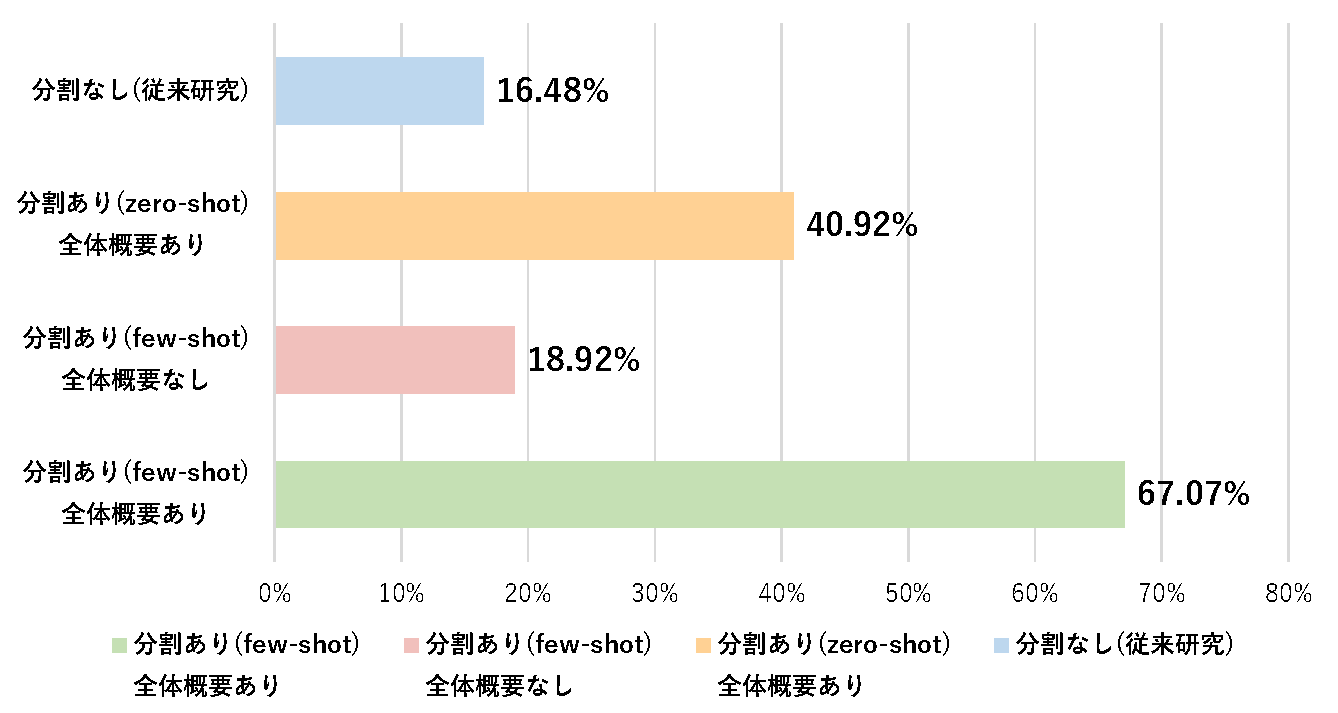
\includegraphics[width=1.0\linewidth]{./Toyoshima_fig/SIGSE_fig1.pdf}
    \caption{マイクロベンチマーク共有サービスの投稿例\protect\footnotemark}
    \label{fig:jsPerf}
\end{figure}
SESで載せた棒グラフ4つのやつ

\subsection{RQ2}
統合前
67.837\% (1,101 / 1,623)

統合後
68.762\% (1,116 / 1,623)

テスト通過率は,統合前・統合後でほぼ横ばいなので劣化は見られない.
\todo{テスト通過率だけじゃなくて,テストが通る問題の分布についても調べる(統合前なら全部通ってたのが,統合後なら通らなくなった,とかを見ていく)}

\subsection{RQ3}
統合前
67.837\% (1,101 / 1,623)

統合後
68.762\% (1,116 / 1,623)

これに対して,テスト通過率
テスト通過率(D問題100問)
85.41666\% (246 / 288)

%6
\section{考察}

%7
\section{妥当性の脅威}

%8
\section{おわりに}
\textbf{謝辞} ありがとうございました

\end{document}

%memo
分割のやり直しでAI-likeな形式に変形された? イテレーション的に回していくコトでAフレンドリーな形式に変形される可能性について考察部分で持っていく